% This file was created by matlab2tikz.
%
%The latest updates can be retrieved from
%  http://www.mathworks.com/matlabcentral/fileexchange/22022-matlab2tikz-matlab2tikz
%where you can also make suggestions and rate matlab2tikz.
%

\pgfplotsset{compat=newest}

\usetikzlibrary{calc}

%%% START MACRO FOR ANNOTATION OF TRIANGLE WITH SLOPE %%%.
\newcommand{\logLogSlopeTriangle}[5]
{
	% #1. Relative offset in x direction.
	% #2. Width in x direction, so xA-xB.
	% #3. Relative offset in y direction.
	% #4. Slope d(y)/d(log10(x)).
	% #5. Plot options.
	
	\pgfplotsextra
	{
		\pgfkeysgetvalue{/pgfplots/xmin}{\xmin}
		\pgfkeysgetvalue{/pgfplots/xmax}{\xmax}
		\pgfkeysgetvalue{/pgfplots/ymin}{\ymin}
		\pgfkeysgetvalue{/pgfplots/ymax}{\ymax}
		
		% Calculate auxilliary quantities, in relative sense.
		\pgfmathsetmacro{\xArel}{#1}
		\pgfmathsetmacro{\yArel}{#3}
		\pgfmathsetmacro{\xBrel}{#1-#2}
		\pgfmathsetmacro{\yBrel}{\yArel}
		\pgfmathsetmacro{\xCrel}{\xArel}
		%\pgfmathsetmacro{\yCrel}{ln(\yC/exp(\ymin))/ln(exp(\ymax)/exp(\ymin))} % REPLACE THIS EXPRESSION WITH AN EXPRESSION INDEPENDENT OF \yC TO PREVENT THE 'DIMENSION TOO LARGE' ERROR.
		
		\pgfmathsetmacro{\lnxB}{\xmin*(1-(#1-#2))+\xmax*(#1-#2)} % in [xmin,xmax].
		\pgfmathsetmacro{\lnxA}{\xmin*(1-#1)+\xmax*#1} % in [xmin,xmax].
		\pgfmathsetmacro{\lnyA}{\ymin*(1-#3)+\ymax*#3} % in [ymin,ymax].
		\pgfmathsetmacro{\lnyC}{\lnyA-#4*(\lnxA-\lnxB)}
		\pgfmathsetmacro{\yCrel}{\lnyC-\ymin)/(\ymax-\ymin)} % THE IMPROVED EXPRESSION WITHOUT 'DIMENSION TOO LARGE' ERROR.
		
		% Define coordinates for \draw. MIND THE 'rel axis cs' as opposed to the 'axis cs'.
		\coordinate (A) at (rel axis cs:\xArel,\yArel);
		\coordinate (B) at (rel axis cs:\xBrel,\yBrel);
		\coordinate (C) at (rel axis cs:\xCrel,\yCrel);
		
		% Draw slope triangle.
		\draw[#5]   (A)-- node[pos=0.5,anchor=south] {\scriptsize 1}
		(B)-- 
		(C)-- node[pos=0.5,anchor=west] {\scriptsize #4}
		cycle;
	}
}
%%% END MACRO FOR ANNOTATION OF TRIANGLE WITH SLOPE %%%.

\newcommand{\logLogSlopeReverseTriangle}[5]
{
	% #1. Relative offset in x direction.
	% #2. Width in x direction, so xA-xB.
	% #3. Relative offset in y direction.
	% #4. Slope d(y)/d(log10(x)).
	% #5. Plot options.
	
	\pgfplotsextra
	{
		\pgfkeysgetvalue{/pgfplots/xmin}{\xmin}
		\pgfkeysgetvalue{/pgfplots/xmax}{\xmax}
		\pgfkeysgetvalue{/pgfplots/ymin}{\ymin}
		\pgfkeysgetvalue{/pgfplots/ymax}{\ymax}
		
		% Calculate auxilliary quantities, in relative sense.
		\pgfmathsetmacro{\xArel}{#1}
		\pgfmathsetmacro{\yArel}{#3}
		\pgfmathsetmacro{\xBrel}{#1+#2}
		\pgfmathsetmacro{\yBrel}{\yArel}
		\pgfmathsetmacro{\xCrel}{\xArel}
		%\pgfmathsetmacro{\yCrel}{ln(\yC/exp(\ymin))/ln(exp(\ymax)/exp(\ymin))} % REPLACE THIS EXPRESSION WITH AN EXPRESSION INDEPENDENT OF \yC TO PREVENT THE 'DIMENSION TOO LARGE' ERROR.
		
		\pgfmathsetmacro{\lnxB}{\xmin*(1-(#1-#2))+\xmax*(#1-#2)} % in [xmin,xmax].
		\pgfmathsetmacro{\lnxA}{\xmin*(1-#1)+\xmax*#1} % in [xmin,xmax].
		\pgfmathsetmacro{\lnyA}{\ymin*(1-#3)+\ymax*#3} % in [ymin,ymax].
		\pgfmathsetmacro{\lnyC}{\lnyA+#4*(\lnxA-\lnxB)}
		\pgfmathsetmacro{\yCrel}{\lnyC-\ymin)/(\ymax-\ymin)}
		
		% Define coordinates for \draw. MIND THE 'rel axis cs' as opposed to the 'axis cs'.
		\coordinate (A) at (rel axis cs:\xArel,\yArel);
		\coordinate (B) at (rel axis cs:\xBrel,\yBrel);
		\coordinate (C) at (rel axis cs:\xCrel,\yCrel);
		
		% Draw slope triangle.
		\draw[#5]   (A)-- node[pos=0.5,anchor=north] {\scriptsize 1}
		(B)-- 
		(C)-- node[pos=0.5,anchor=east] {\scriptsize #4}
		cycle;
	}
}
%%% END MACRO FOR ANNOTATION OF TRIANGLE WITH SLOPE %%%.

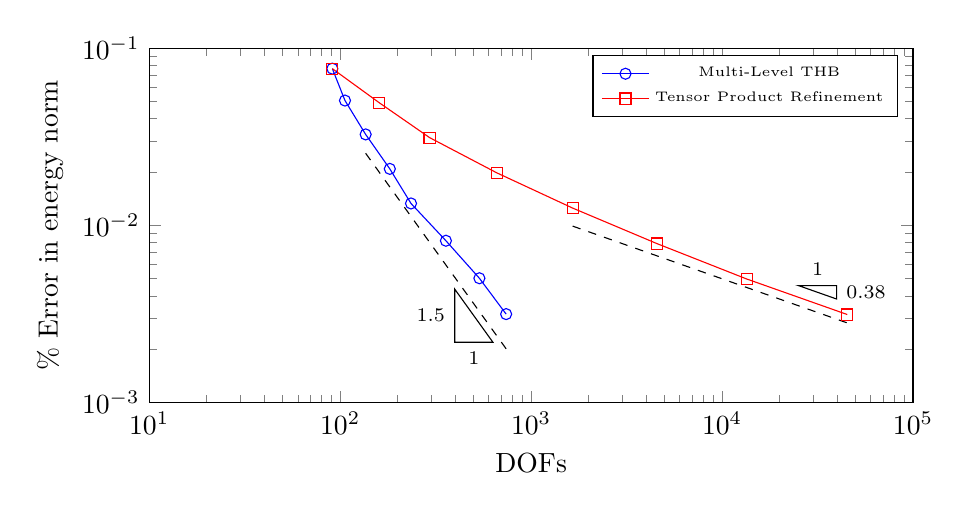
\begin{tikzpicture}

\begin{axis}[%
width=0.8\textwidth,
height=4.5cm,
at={(0in,0in)},
scale only axis,
xmode=log,
xmin=10,
xmax=1e5,
xminorticks=true,
ymode=log,
ymin=1e-3,
ymax=0.1,
yminorticks=true,
axis background/.style={fill=white},
ylabel=\% Error in energy norm,
xlabel=DOFs,
legend style={font=\tiny}
]
\addplot [color=blue,solid,mark=o,mark options={solid}]
table[row sep=crcr]{%
	91	0.076639669632431\\
	106	0.050619991986389\\
	136	0.03259996732911\\
	182	0.020829831705275\\
	235	0.013288521039441\\
	358	0.008185330345575\\
	536	0.005026862415664\\
	740	0.003154704476209\\
};
\addplot [color=black,dashed,forget plot]
table[row sep=crcr]{%
%	91	0.0465937316999286\\
%	106	0.0370621649956555\\
	136	0.0255024098183088\\
	182	0.016473371822903\\
	235	0.0112276221759187\\
	358	0.00597124709593732\\
	536	0.00325943555378186\\
	740	0.00200928713444596\\
};

\addplot [color=red,solid,mark=square,mark options={solid}]
table[row sep=crcr]{%
	91	0.0766396696324313\\
	160	0.0492573753694321\\
	294	0.0312745259781169\\
	660	0.0198067026806826\\
	1650	0.0125150519229291\\
	4550	0.00789625154842711\\
	13464	0.00497832932312483\\
	45257	0.00313741507918149\\
};
\addplot [color=black,dashed,forget plot]
table[row sep=crcr]{%
	%91	0.0297737956632537\\
	%160	0.0240272650477109\\
%	294	0.0190676840468274\\
%	660	0.0140230743631824\\
	1650	0.00989979117577662\\
	4550	0.00673326336563706\\
	13464	0.00445844869525894\\
	45257	0.00281260887622936\\
};

\legend{Multi-Level THB, Tensor Product Refinement}

	\logLogSlopeReverseTriangle{0.4}{0.05}{0.17}{1.5}{black};
    \logLogSlopeTriangle{0.9}{0.05}{0.33}{0.38}{black};
\end{axis}
\end{tikzpicture}%